\section{Experiments}
We evaluate the VR bound methods on Bayesian neural networks and variational auto-encoders. The implementation of all the experiments in Python is released at \url{https://github.com/YingzhenLi/VRbound}.

\subsection{Bayesian neural networks}

The first experiment considers Bayesian neural network regression. The datasets are collected from the UCI dataset repository.\footnote{\url{http://archive.ics.uci.edu/ml/datasets.html}} We use a Gaussian prior $\bm{\theta} \sim \mathcal{N}(\bm{\theta}; \bm{0}, \bm{I})$ for the network weights and Gaussian approximation to the true posterior $q(\bm{\theta}) = \mathcal{N}(\bm{\theta}; \bm{\mu}_q, diag(\bm{\sigma}_q))$. We fit the parameters of $q$ and the noise level $\sigma$ by optimising the lower-bound. We follow the toy example in Section \ref{sec:vr_bound} and consider $\alpha \in \{-\infty, 0.0, 0.5, 1.0, +\infty \}$ in order to examine the effect of mass-covering/zero-forcing behaviour. Stochastic optimisation uses the energy approximation strategy proposed in Section \ref{sec:chap4_vrbound_large_scale_learning}. 

For regression tests, we consider Protein and Year as the large datasets and the remainder as small datasets. For all small datasets we used single-layer neural networks with 50 hidden units (ReLUs), and for Protein and Year we used 100 units. The methods for comparison were run for $500$ epochs on the small datasets and $100$, $40$ epochs for the large datasets, respectively. We used ADAM \citep{kingma:adam2015} for optimisation with learning rate 0.001 and the standard setting for other parameters. For stochastic optimisation we used mini-batch size $M = 32$ and number of MC samples $K=100$ and $K=10$ for small and large datasets, respectively. The number of dataset random splits is 20 except for the large datasets, which is 5 and 1 for Protein and Year, respectively. 

\begin{figure}[t]
\centering
    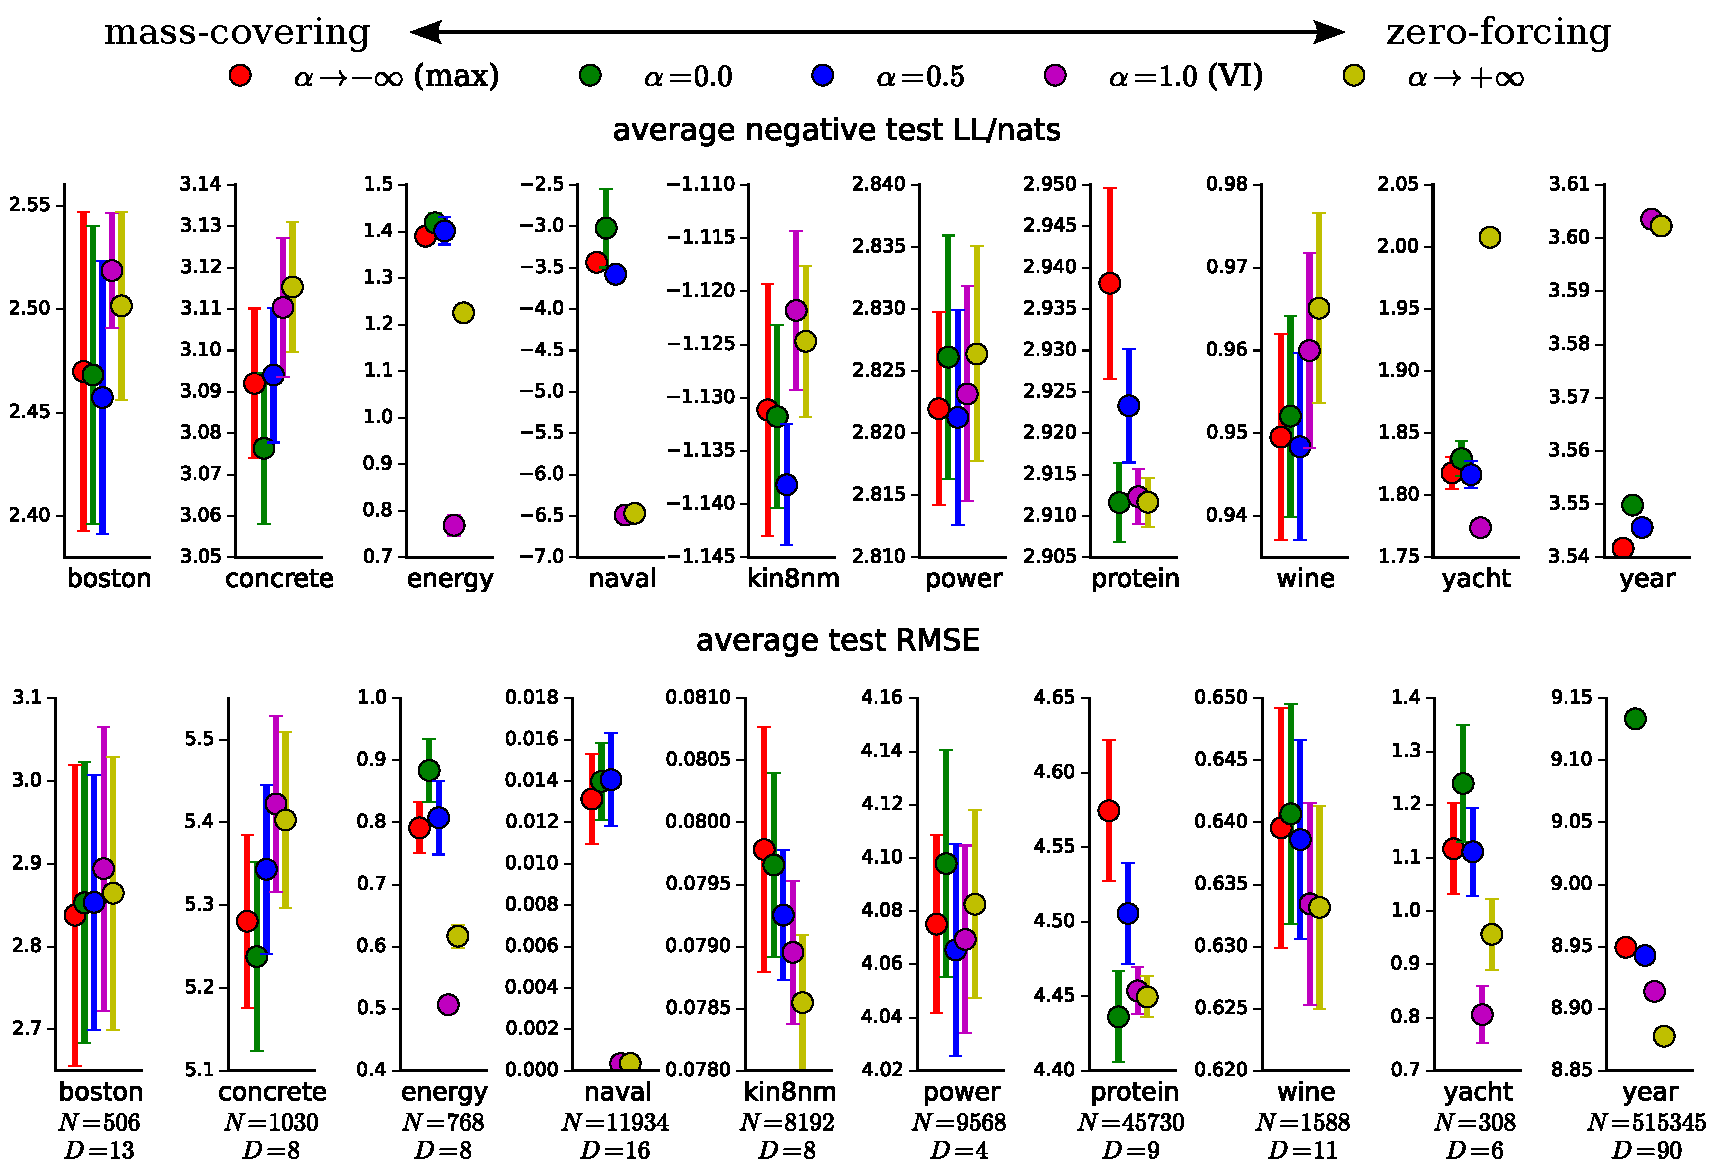
\includegraphics[width=1\linewidth]{Chapter4/vrbound/figs/results_all_bnn}
    \caption{Test LL and RMSE results for Bayesian neural network regression. The lower the better. The error bars show 1-standard deviation across 20 random splits of the data.}
    \label{fig:chap4_vrbound_bnn_results_all}
\end{figure}
%
\begin{figure}
%\begin{table}[ht]
\centering
\captionof{table}{Regression experiment: Average negative test log likelihood/nats}
\label{tab:chap4_vrbound_bnn_ll}
\begin{tabular}{l@{\ica}r@{\ica}r@{\ica}r@{$\pm$}l@{\ica}r@{$\pm$}l@{\ica}r@{$\pm$}l@{\ica}r@{$\pm$}l@{\ica}r@{$\pm$}l@{\ica}}
\hline
\bf{Dataset}&{N}&{D}&\multicolumn{2}{c}{\bf{$\alpha \rightarrow -\infty$}}&\multicolumn{2}{c}{\bf{$\alpha = 0.0$}}&\multicolumn{2}{c}{\bf{$\alpha = 0.5$}}&\multicolumn{2}{c}{\bf{$\alpha = 1.0$ (VI)}}&\multicolumn{2}{c}{\bf{$\alpha \rightarrow +\infty$}}\\
\hline
boston&506&13&2.47&0.08&2.47&0.07&\underline{\textit{2.46}}&\underline{\textit{0.07}}&\textbf{2.52}&\textbf{0.03}&2.50&0.05\\
concrete&1030&8&3.09&0.02&\underline{\textit{3.08}}&\underline{\textit{0.02}}&3.09&0.02&3.11&0.02&\textbf{3.12}&\textbf{0.02}\\
energy&768&8&1.39&0.02&\textbf{1.42}&\textbf{0.02}&1.40&0.03&\underline{\textit{0.77}}&\underline{\textit{0.02}}&1.23&0.01\\
naval&11934&16&-3.43&0.08&\textbf{-3.02}&\textbf{0.48}&-3.58&0.08&\underline{\textit{-6.49}}&\underline{\textit{0.04}}&-6.47&0.09\\
kin8nm&8192&8&-1.13&0.01&-1.13&0.01&\underline{\textit{-1.14}}&\underline{\textit{0.01}}&\textbf{-1.12}&\textbf{0.01}&-1.12&0.01\\
power&9568&4&2.82&0.01&2.83&0.01&\underline{\textit{2.82}}&\underline{\textit{0.01}}&2.82&0.01&\textbf{2.83}&\textbf{0.01}\\
protein&45730&9&\textbf{2.94}&\textbf{0.01}&\underline{\textit{2.91}}&\underline{\textit{0.00}}&2.92&0.01&2.91&0.00&2.91&0.00\\
wine&1588&11&0.95&0.01&0.95&0.01&\underline{\textit{0.95}}&\underline{\textit{0.01}}&0.96&0.01&\textbf{0.97}&\textbf{0.01}\\
yacht&308&6&1.82&0.01&1.83&0.01&1.82&0.01&\underline{\textit{1.77}}&\underline{\textit{0.01}}&\textbf{2.01}&\textbf{0.00}\\
year&515345&90&\underline{\textit{3.54}}&NA&3.55&NA&3.55&NA&\textbf{3.60}&NA&3.60&NA\\
\hline
\multicolumn{3}{c}{\textbf{Average Rank}}&2.80&0.34&3.00&0.45&\textbf{2.20}&\textbf{0.37}&3.20&0.51&3.80&0.39\\
\hline
\end{tabular}
%\end{table}

%\begin{table}[ht]
\centering
\captionof{table}{Regression experiment: Average test RMSE}
\label{tab:chap4_vrbound_bnn_rmse}
\begin{tabular}{l@{\ica}r@{\ica}r@{\ica}r@{$\pm$}l@{\ica}r@{$\pm$}l@{\ica}r@{$\pm$}l@{\ica}r@{$\pm$}l@{\ica}r@{$\pm$}l@{\ica}}
\hline
\bf{Dataset}&{N}&{D}&\multicolumn{2}{c}{\bf{$\alpha \rightarrow -\infty$}}&\multicolumn{2}{c}{\bf{$\alpha = 0.0$}}&\multicolumn{2}{c}{\bf{$\alpha = 0.5$}}&\multicolumn{2}{c}{\bf{$\alpha = 1.0$ (VI)}}&\multicolumn{2}{c}{\bf{$\alpha \rightarrow +\infty$}}\\
\hline
boston&506&13&\underline{\textit{2.84}}&\underline{\textit{0.18}}&2.85&0.17&2.85&0.15&\textbf{2.89}&\textbf{0.17}&2.86&0.17\\
concrete&1030&8&5.28&0.10&\underline{\textit{5.24}}&\underline{\textit{0.11}}&5.34&0.10&\textbf{5.42}&\textbf{0.11}&5.40&0.11\\
energy&768&8&0.79&0.04&\textbf{0.88}&\textbf{0.05}&0.81&0.06&\underline{\textit{0.51}}&\underline{\textit{0.01}}&0.62&0.02\\
naval&11934&16&0.01&0.00&0.01&0.00&\textbf{0.01}&\textbf{0.00}&\underline{\textit{0.00}}&\underline{\textit{0.00}}&0.00&0.00\\
kin8nm&8192&8&\textbf{0.08}&\textbf{0.00}&0.08&0.00&0.08&0.00&0.08&0.00&\underline{\textit{0.08}}&\underline{\textit{0.00}}\\
power&9568&4&4.08&0.03&\textbf{4.10}&\textbf{0.04}&\underline{\textit{4.07}}&\underline{\textit{0.04}}&4.07&0.04&4.08&0.04\\
protein&45730&9&\textbf{4.57}&\textbf{0.05}&\underline{\textit{4.44}}&\underline{\textit{0.03}}&4.51&0.03&4.45&0.02&4.45&0.01\\
wine&1588&11&0.64&0.01&\textbf{0.64}&\textbf{0.01}&0.64&0.01&0.63&0.01&\underline{\textit{0.63}}&\underline{\textit{0.01}}\\
yacht&308&6&1.12&0.09&\textbf{1.24}&\textbf{0.11}&1.11&0.08&\underline{\textit{0.81}}&\underline{\textit{0.05}}&0.96&0.07\\
year&515345&90&8.95&NA&\textbf{9.13}&NA&8.94&NA&8.91&NA&\underline{\textit{8.88}}&NA\\
\hline
\multicolumn{3}{c}{\textbf{Average Rank}}&3.40&0.38&3.70&0.51&3.20&0.31&2.40&0.45&\textbf{2.30}&\textbf{0.38}\\
\hline
\end{tabular}
%\end{table}

       
\end{figure}

We summarise the test negative log-likelihood (LL) and RMSE with standard error (across different random splits except for Year) for selected datasets in Figure \ref{fig:chap4_vrbound_bnn_results_all} and Table \ref{tab:chap4_vrbound_bnn_ll}, \ref{tab:chap4_vrbound_bnn_rmse}. In the tables the best performing results are underlined, while the worse cases are also bold-faced. These results indicate that for posterior approximation problems, the optimal $\alpha$ may vary for different datasets (although for Boston and Power the performances are very similar). 
%

It can be particularly tricky to approximate the posterior distribution of the weight matrices for a neural network. Since one can obtain the same output by swapping the positions of two hidden units and adjusting the corresponding in- and out-going weights, there exist symmetric modes in the exact posterior of the weight matrices. In this case mass-covering can be harmful, e.g.~for Naval and Energy datasets, methods with $\alpha < 1.0$ values seem to be under-performing, not only for predictive error but also for test log-likelihood measure. 
But still, we observed two major trends. Zero-forcing/mode-seeking methods tend to focus on improving the predictive error. Mass-covering methods, on the other hand, returns better test log-likelihood, which has been shown empirically to be correlated with the quality of the approximated uncertainty estimate \citep{hernandez-lobato:pbp2015, gal:uncertainty2016, depeweg:bnn_rl2016}. In particular VI returns lower test log-likelihood for most of the datasets. Furthermore, $\alpha = 0.5$ produced overall good results for both test LL and RMSE, possibly because the skew symmetry is centred at $\alpha = 0.5$ and the corresponding divergence is the only symmetric distance measure in the family. Future work should develop algorithms to automatically select the best $\alpha$ values, although a naive approach could use validation sets. 

\subsection{Variational auto-encoders}

The second experiments considers variational auto-encoders for unsupervised learning. We mainly compare three approaches: VAE ($\alpha = 1.0$), IWAE ($\alpha = 0$), and VR-max ($\alpha = -\infty$), which are implemented upon the publicly available code.\footnote{\url{https://github.com/yburda/iwae}}
%
Four datasets are considered: Frey Face\footnote{\url{http://www.cs.nyu.edu/~roweis/data.html}} (with 10-fold cross validation), Caltech 101 Silhouettes\footnote{\url{https://people.cs.umass.edu/~marlin/data.shtml}}, MNIST\footnote{\url{http://yann.lecun.com/exdb/mnist/}} and OMNIGLOT\footnote{\url{https://github.com/brendenlake/omniglot}}. The VAE model has $L=1, 2$ stochastic layers with deterministic layers stacked between.  The detailed numbers of stochastic layers $L$, number of hidden units, and the activation function are summarised in Table \ref{tab:vae_arch}. The prefix of the number indicates whether this layer is \textbf{d}eterministic or \textbf{s}tochastic, e.g.~d500-s200 stands for a neural network with one deterministic layer of 500 units followed by a stochastic layer of 200 units. For Frey Face data we train the models using learning rate 0.0005 and mini-batch size 100. For MNIST and OMNIGLOT we reuse the settings from \cite{burda:iwae2016}: the training process runs for $3^i$ passes with learning rate $0.0001 \cdot 10^{-i/7}$ for $i = 0, ..., 7$, and the batch size is 20. For Caltech Silhouettes we use the same settings as MNIST and OMNIGLOT except that the training proceeded for $\sum_{i=0}^7 2^i = 255$ epochs. We reproduce the IWAE experiments to obtain a fair comparison, since the results in the original publication \citep{burda:iwae2016} mismatches those evaluated on the publicly available code.
%

\begin{table}[!ht]
\centering
\captionof{table}{Network architecture of tested VAE algorithms.}
\label{tab:vae_arch}
\begin{tabular}{lccccc}
\hline
\bf{Dataset}&$L$&architecture&activation&probability type (p/q)\\
\hline
Frey Face&1& d200-d200-s20&softplus&Gaussian/Gaussian\\
\hline
Caltech 101& 1&d500-s200&tanh&Bernoulli/Gaussian\\
\hline
MNIST \& & 1&d200-d200-s50&tanh&Bernoulli/Gaussian\\
OMNIGLOT     & 2&d200-d200-s100-d100-d100-s50&tanh&Bernoulli/Gaussian\\
\hline
\end{tabular}
\end{table}

%

\begin{figure}
\begin{minipage}{0.6\linewidth}

%\begin{table}[t]
\centering
%\caption
\captionof{table}{ Average Test log-likelihood. Results for VAE on MNIST and OMNIGLOT are collected from \cite{burda:iwae2016}.}
\label{tab:vae_ll}
\begin{tabular}{lccccc}
\toprule
\bf{Dataset}&$L$&$K$&\bf{ VAE }&\bf{ IWAE }&\bf{ VR-max }\\
\hline
Frey Face&1&5&1322.96&\bf{1380.30}&1377.40\\
($\pm$ std. err.)& & &$\pm$10.03&\bf{$\pm$4.60}&$\pm$4.59 \\
\hline
Caltech 101& 1& 5&-119.69&\bf{-117.89}&-118.01\\
Silhouettes&  &50&-119.61&-117.21&\bf{-117.10}\\
\hline
MNIST& 1&5 &-86.47&\bf{-85.41}&-85.42\\
     &  &50&-86.35&\bf{-84.80}&-84.81\\
     & 2&5 &-85.01&\bf{-83.92}&-84.04\\
     &  &50&-84.78&\bf{-83.05}&-83.44\\
\hline
OMNIGLOT & 1&5 &-107.62&\bf{-106.30}&-106.33\\
		 & 1&50&-107.80&\bf{-104.68}&-105.05\\
		 & 2&5 &-106.31&\bf{-104.64}&-104.71\\
		 & 2&50&-106.30&\bf{-103.25}&-103.72\\
\bottomrule
\end{tabular}
%\end{table}

\end{minipage}
\hfill
\begin{minipage}{0.35\linewidth}
\centering
 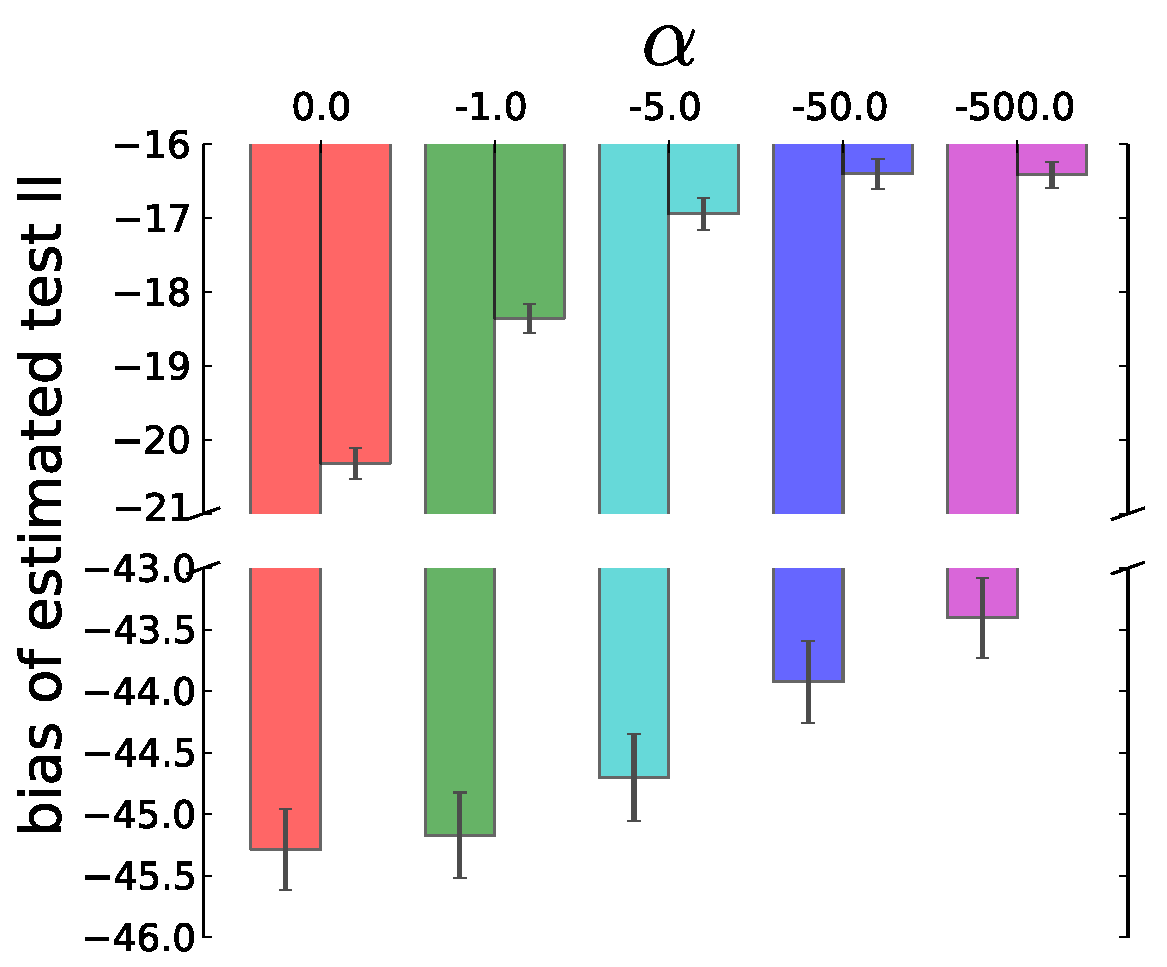
\includegraphics[width=1.00\linewidth]{Chapter4/vrbound/figs/bias_estimate.pdf} 
 \captionof{figure}{Bias of sampling approximation to. Results for $K=5, 50$ samples are shown on the left and right, respectively.}
 \label{fig:vae_bias}
\end{minipage}
\end{figure}
%
\begin{figure*}[!ht]
 \centering
 \subfigure[Log of ratio $R = w_{max} / (1 - w_{max})$]{
 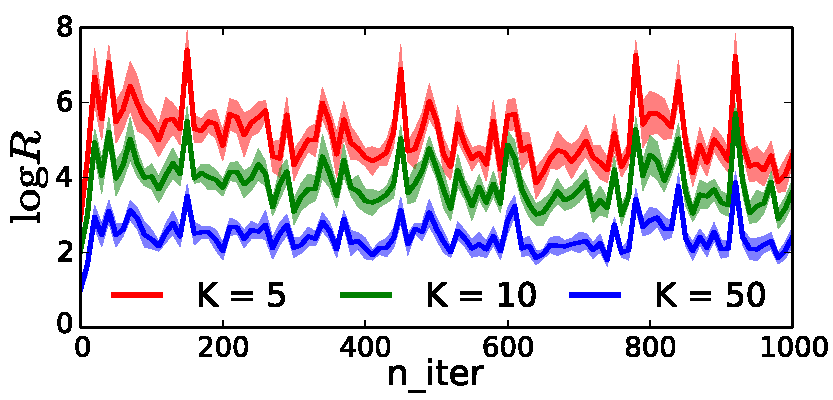
\includegraphics[width=0.37\linewidth]{Chapter4/vrbound/figs/weight_ratio.pdf}
 \label{fig:weight_ratio}}
 \hspace{0.4in}
 \subfigure[Weights of samples.]{
 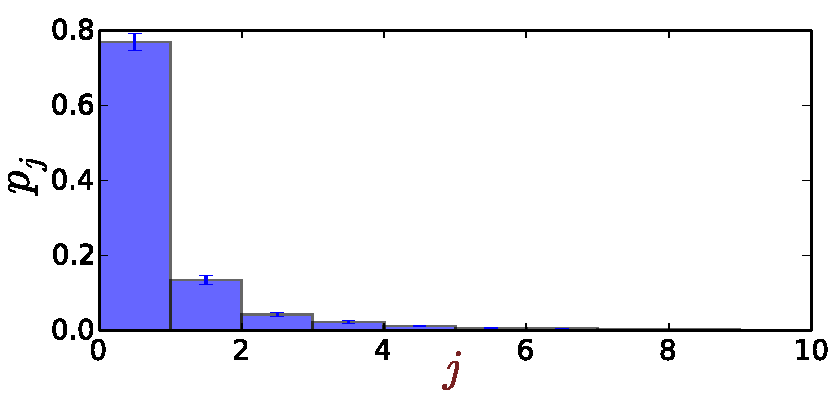
\includegraphics[width=0.37\linewidth]{Chapter4/vrbound/figs/weight_distribution.pdf}
 \label{fig:weight_distribution}}
 \caption{Importance weights during training, see main text for details. Best viewed in colour.}
\end{figure*}

We report test log-likelihood results in Table \ref{tab:vae_ll} by computing $\log p(\bm{x}) \approx \hat{\mathcal{L}}_{0, 5000}(q; \bm{x})$ following \cite{burda:iwae2016}. We also present some samples from the VR-max trained auto-encoders in Figure \ref{fig:vae_samples}.
%
\begin{figure}
 \centering
  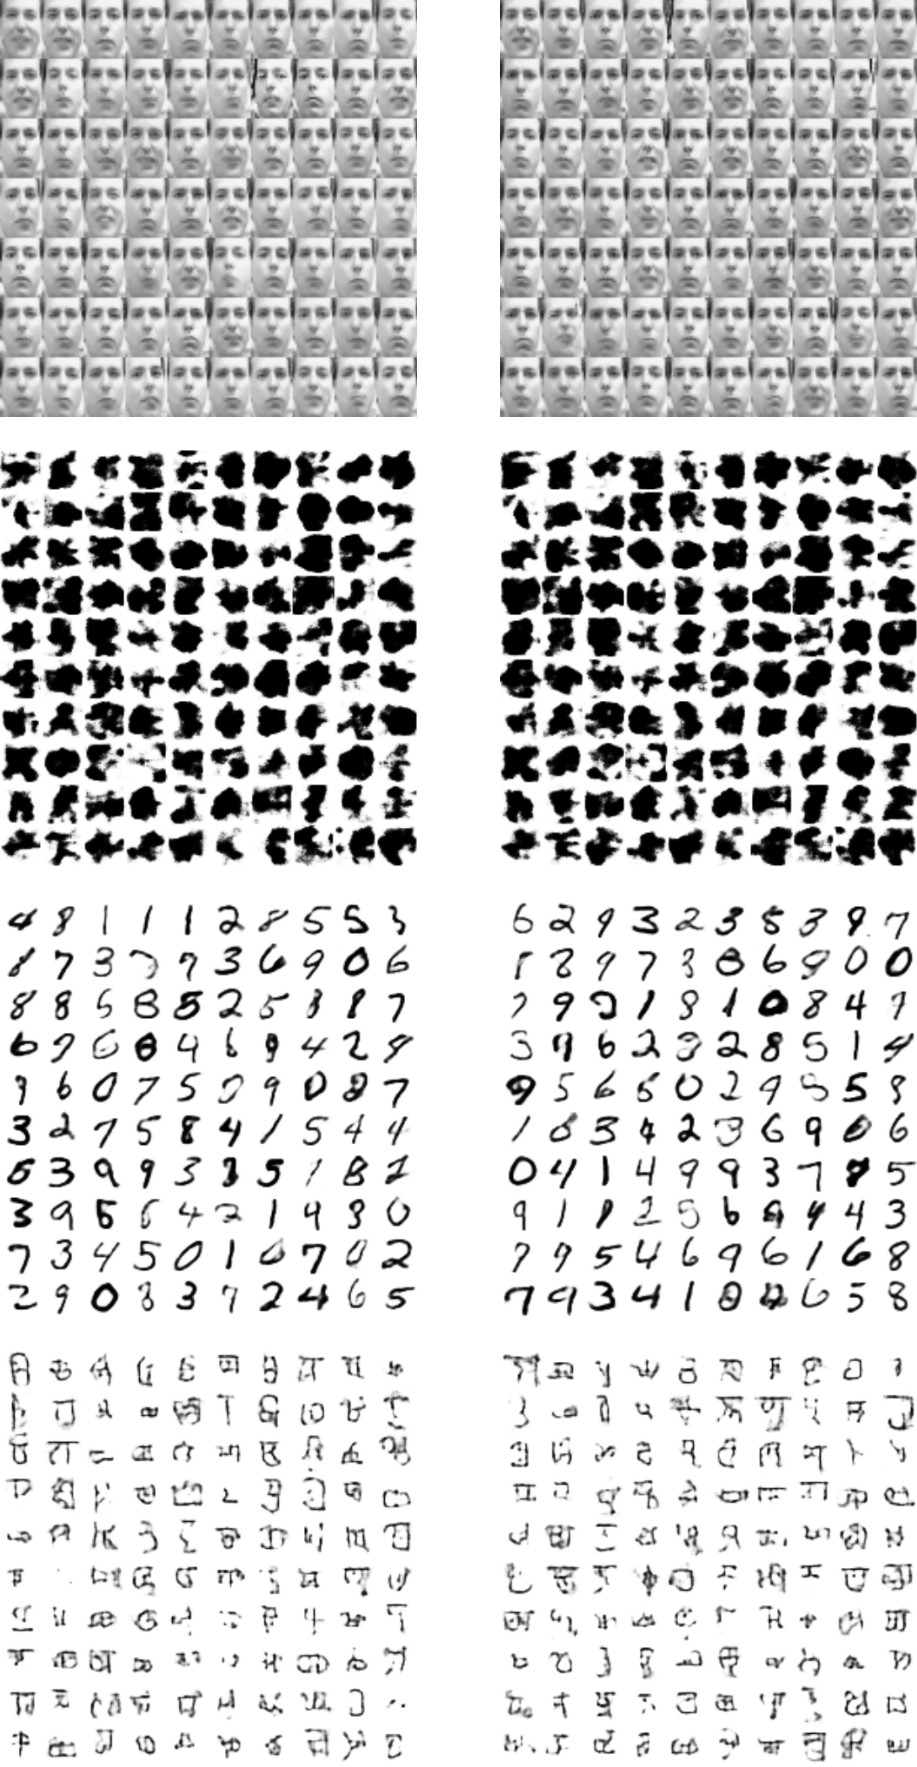
\includegraphics[width=0.6\linewidth]{Chapter4/vrbound/figs/vae_samples.pdf}
  \caption{Sampled images from the the best models trained with IWAE (left) and VR-max (right).}
  \label{fig:vae_samples}
\end{figure}
%
Overall VR-max is almost indistinguishable from IWAE. Other positive alpha settings (e.g.~$\alpha = 0.5$) return worse results, e.g. $1374.64\pm5.62$ for Frey Face and $-85.50$ for MNIST with $\alpha = 0.5$, $L=1$ and $K=5$. These worse results for $\alpha > 0$ indicate the preference of getting tighter approximations to the likelihood function for MLE problems. Small negative $\alpha$ values (e.g.~$\alpha = -1.0, -2.0$) return better results on different splits of the Frey Face data, and overall the best $\alpha$ value is dataset-specific.\footnote{Since presentation of this work at NIPS 2016, \cite{bui:dgm2016} revisited this idea with slightly different architecture set-up, and showed that $\alpha \neq 0$ values are usually favoured over the IWAE approach. }

VR-max's success might be explained by the tightness of the bound. To evaluate this, we compute the VR bounds on $100$ test datapoints using the 1-layer VAE trained on Frey Face, with $K=\{5, 50\}$ and $\alpha \in \{0, -1, -5, -50, -500 \}$. Figure \ref{fig:vae_bias} presents the estimated gap $\hat{\mathcal{L}}_{\alpha, K} - \hat{\mathcal{L}}_{0, 5000}$. The results indicates that $\hat{\mathcal{L}}_{\alpha, K}$ provides a lower-bound, agreeing with the theoretical results presented in Section \ref{sec:chap4_vrbound_sampling}, and that gap is narrowed as $\alpha \rightarrow -\infty$. Also increasing $K$ provides improvements. The standard error of estimation is almost constant for different $\alpha$ (with $K$ fixed), and is negligible when compared to the MC approximation bias.

%
Another explanation for VR-max's success is that, the sample with the largest normalised importance weight $w_{max}$ dominates the contributions of all the gradients.
This is confirmed by tracking $R = \frac{w_{max}}{1 - w_{max}}$ during training on Frey Face (Figure \ref{fig:weight_ratio}). Also Figure \ref{fig:weight_distribution} shows the $10$ largest importance weights from $K=50$ samples in descending order, which exhibit an exponential decay behaviour, with the largest weight occupying more than $75\%$ of the probability mass. This means, the IWAE algorithm is not efficient in terms of sample efficiency, since the learning signal from back-propagation is dominated by the gradients computed on the particle with the largest weight.
%
It also indicates that, VR-max can provide a fast approximation to IWAE when tested on CPUs or multiple GPUs with high communication costs. Indeed our numpy implementation of VR-max achieves up to a 3 times speed-up compared to IWAE (9.7s vs.~29.0s per epoch, tested on Frey Face data with $K = 50$ and batch size $M = 100$, CPU info: Intel Core i7-4930K CPU @ 3.40GHz). However this speed advantage is less significant when the gradients can be computed very efficiently on a single GPU.